\subsection{Integrating deduplication, caching, and Docker registries}
\label{sec:design}

%\sysname\ performs file-level deduplication for a Docker registry.
%
\begin{figure*}[t]
	\centering
		%\begin{minipage}{0.225\textwidth}
			\centering
			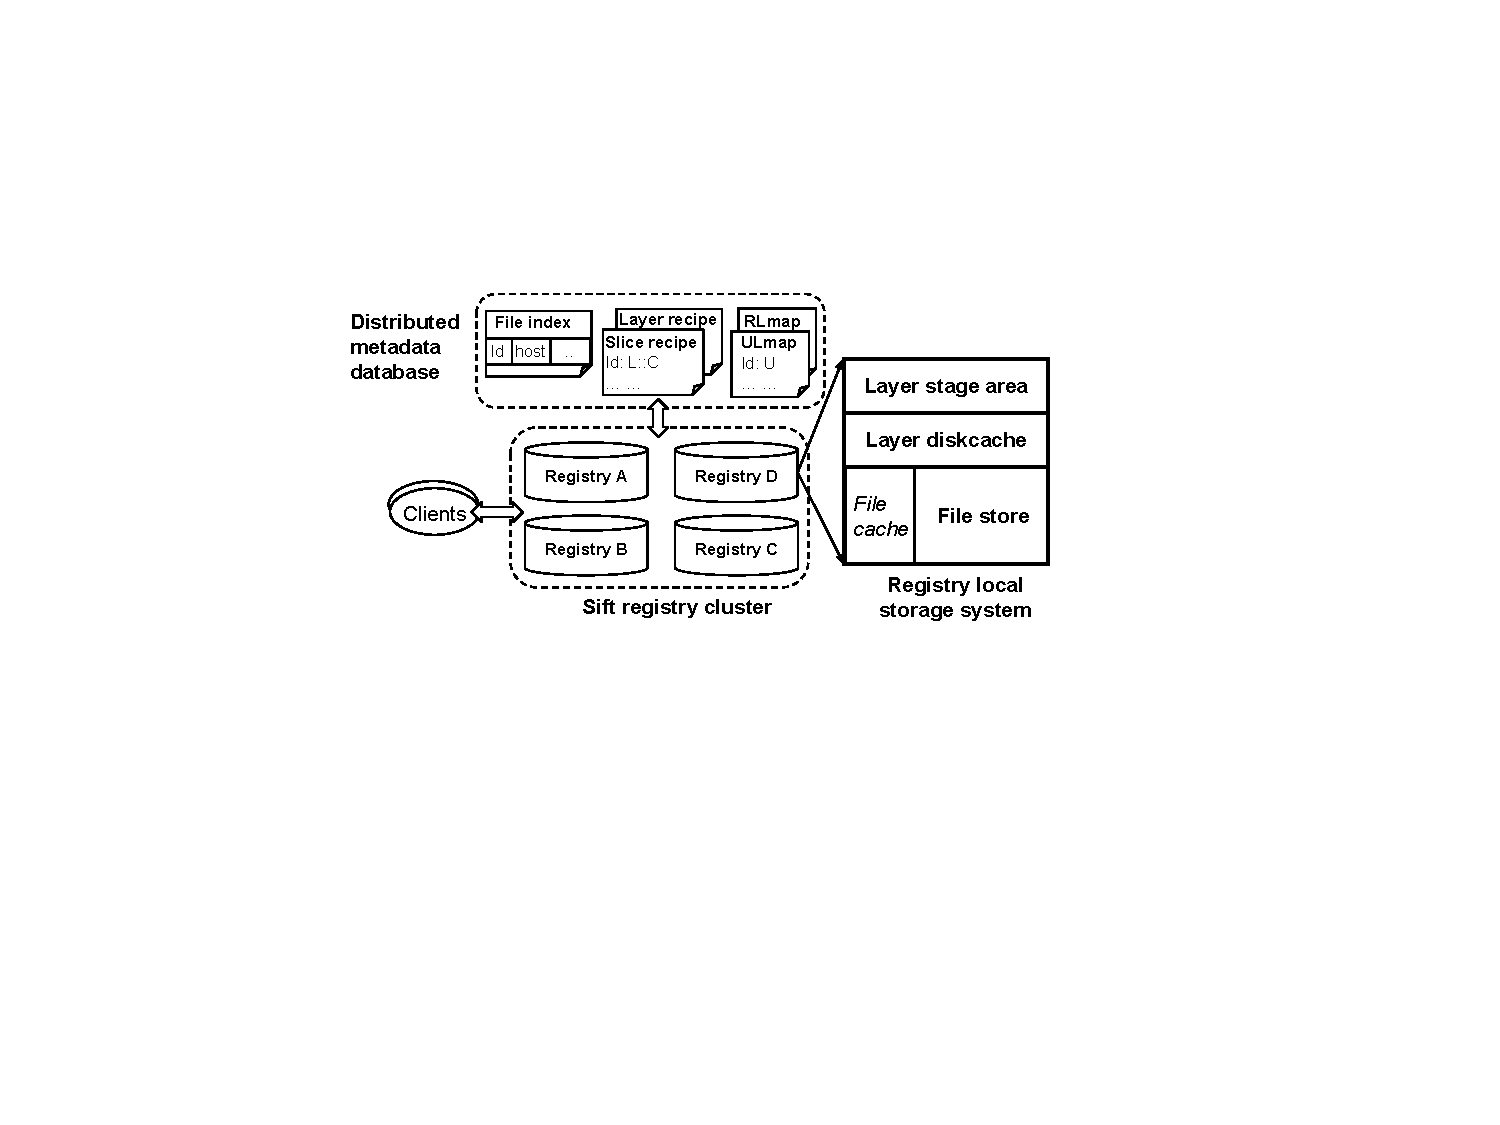
\includegraphics[width=0.9\textwidth]{graphs/sys-architecture.pdf}
%\vspace{-4pt}
			\caption{Architecture of \sysname.}
			%\label{fig:ref_count}
		%\end{minipage}
%	\begin{minipage}{0.225\textwidth}
%		\centering
%		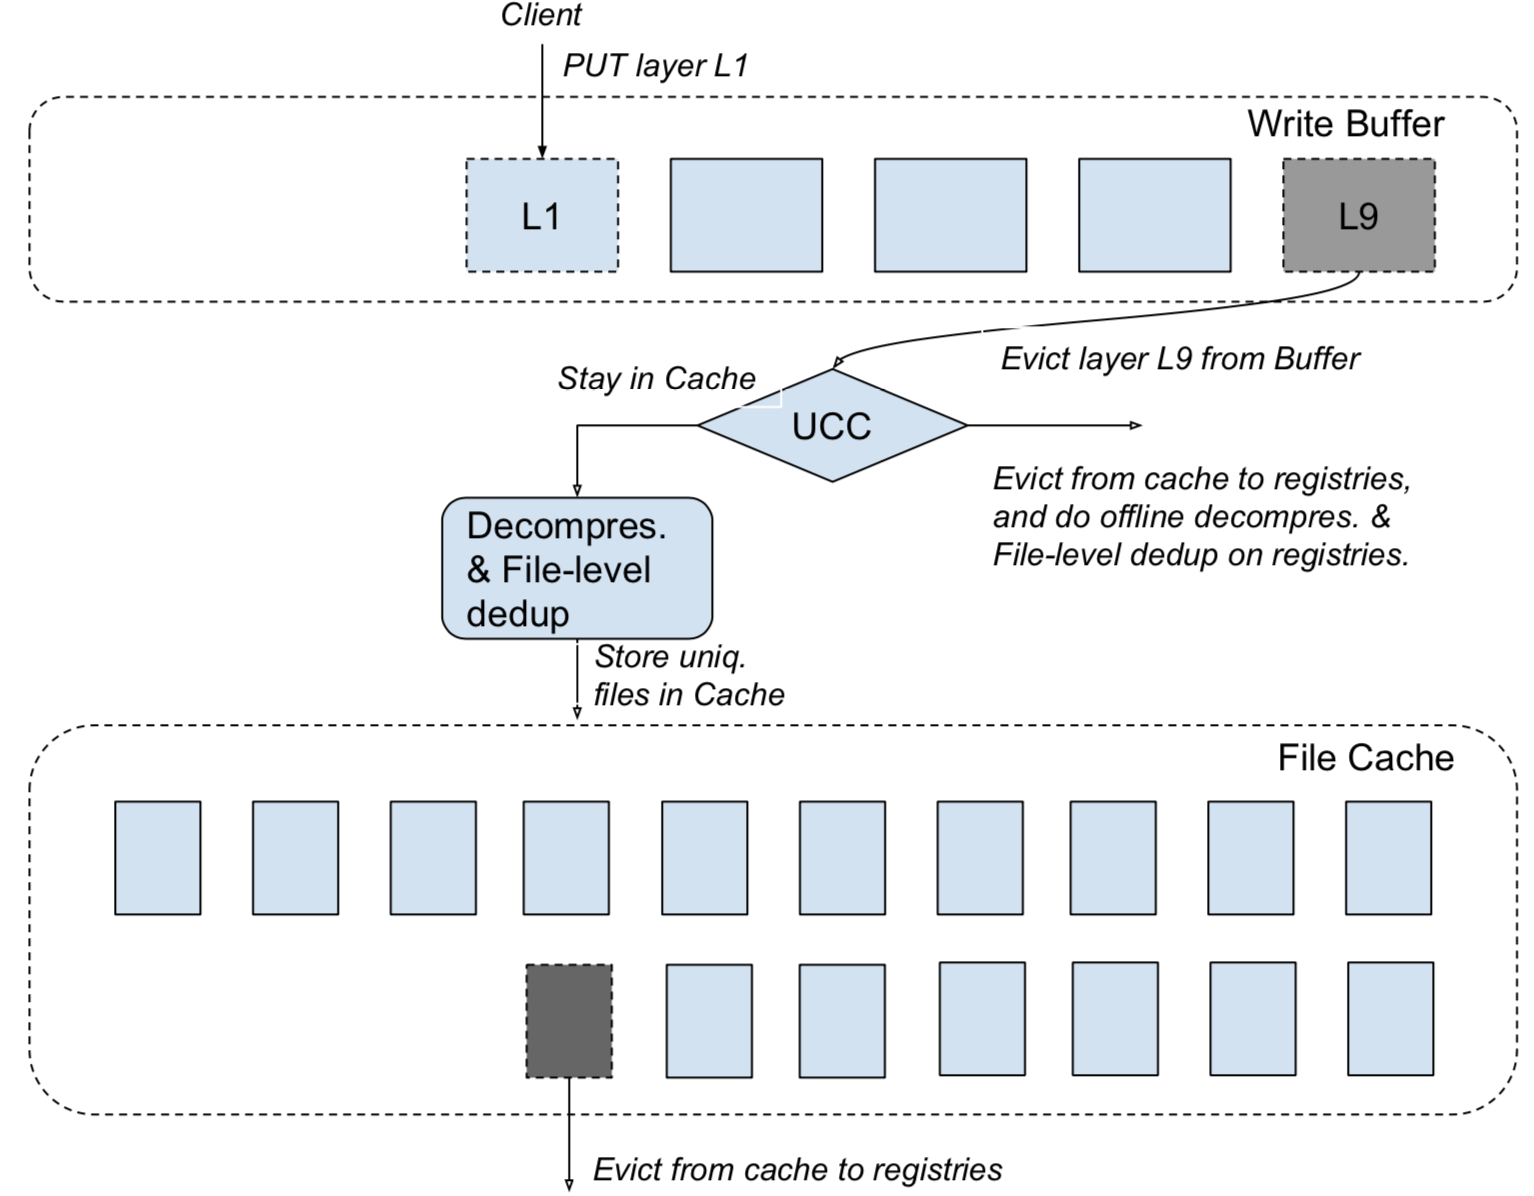
\includegraphics[width=1\textwidth]{graphs/slimmer-cache.png}
%		\caption{CDF of compress. and uncompress. layer size.}
%		\vspace{-3pt}
		\label{fig:sys-overview}
%\vspace{-4pt}
%	\end{minipage}
\end{figure*}

%We designed \sysname\ so that the interface between the Docker clients and the
%registry remains unchanged.
%
%As such, no modifications to the Docker clients are needed.
%
%Below we describe how \sysname\ handles layer pushes and
%pulls at the registry side.
%
%For the sake of this paper, we explain only the main steps omitting smaller
%details.
%\Ali{Following text makes no sense.. what are you trying to explain??}
%\NZ{This part includes our architecture. Our architecture doesn't required many words to explain}
%
%Traditionally, Docker registry is a web server that serves Docker
%\texttt{pull} and Docker \texttt{push} requests.  Although Docker registry is a
%layer-level content addressable storage system holding all the images, it
%delegates storage to drivers which interact with either a local file system or
%a remote cloud storage like S3~\cite{xxx}, Microsoft Azure~\cite{xxxx}, OpenStack Swift~\cite{xxx}, and Aliyun
%OSS~\cite{xxx} as shown in Figure~\ref{fig:sys-overview}.
%Deduplication methods are implemented on remote cloud storage servers or data centers to
%transparently remove duplicates from the incoming data stream.

%proxy caches, or web/HTTP caches 
%Modern container registries such as Google Container Registry~\cite{GoogleContainerRegistry} use cloud storage as their backend Docker image storage systems. 
%Users push and pull Docker images to and from their repositories stored on cloud storage. 
%
%To facilitate a fast and high-availability service, container registries use regional private repositories across the world.  
%This geographical distribution allows users to store images close to their compute instances and experience a fast response time. 
%For example, IBM's Container Registry setup spans five regions~\cite{dockerworkload}. 

%caches are placed as close to the requesting client as possible,
%such caches are known as for the temporary
%storage of frequently requested data to reduce the server's lag.  They are
%typically deployed in a regional ISP or within a corporate network.

\sysname~seamlessly integrates 
%the management of 
a cache along with a deduplication mechanism on the
backend storage system, that we call \emph{backend dedup storage}, with Docker registries
%\Ali{Following information should be part of Background section..
%Intuitively, registries can be deployed as a proxy cache to host
%frequently requested layers.  This approach, a registry as a pull-through
%cache, speeds up image pulls and improves overall performance.  At the same
%time, the backend cloud storage can leverage deduplication to save storage
%space.}\NZ{moved}
%A traditional backend dedup storage cannot meet registry performance requirement
%especially for \texttt{pull} requests due to the large overhead during layer restoring. 
%\subsection{Design challenges}
\sysname~addresses the unique challenges concerning such integration.
%of caching and deduplication to the Docker registry.
First, for caching layers, \texttt{pull} layer requests are difficult to
predict because same layers are not accessed frequently.
We observed that, around half of the cached layers' are not
accessed again for at least 1.3 hours which means that if we
cache a layer, we might need to wait hours to get a hit on that layer as mentioned in Section~\cref{sec:background}.  
This is
because when a user pulls an image from the registry, the Docker daemon on the
requesting host will only pull the layers that are not locally stored.
%\Ali{I do not understand the following sentence.}
%Moreover, we have to consider that a user might deploy an applications on
%multiple machines, so it's not easy to predict when a user will access which layers. 
Ali Anwar et
al., proposed a prefetching method~\cite{dockerworkload} based on the
\texttt{push}-\texttt{pull} relationship: when there is a \texttt{PUSH} layer
request directly followed by a \texttt{GET} manifest request, a \texttt{GET}
layer request will most probably follow. 
However, based on our trace analysis in~\cref{sec:background},
only half of the \texttt{GET} layer
requests have a precedent \texttt{PUSH} layer request within the trace
%collecting duration
collection period of 75 days. This means that, after a user pushes a layer
to the registry, it takes a few days, weeks, or even months for a user to make
a \texttt{pull} request.
%%\Ali{The above statement is incorrect. You have to distinguish between GET layer requests
%that are issued after a (PUSH layer + GET manifest) request and a normal GET layer request.
%FAST paper only talk about case 1. Whereas you are generalizing that any GET layer request
%should have a precedent GET layer request which is wrong. We can make a case
%that not all GET layers requests have a precedent PUSH layer request but we can
%not say that it takes a few days, weeks, or even months for a user to make a pull
%layer request after a push layer request.}
%\NZ{I mean the first case, push beyond your trace collection time.}
%
Second, we can not deduplicate compressed layers. Hence, for deduplication each layer
needs to be uncompressed and then undergo a file-level deduplication. Similarly,
to restore a layer, we need to fetch files from multiple servers and then compress
them in to a tar file. 
This whole process can cause a 
considerable overhead on \texttt{pull} layer requests performance.
Deduplication also slows down
\texttt{push} layer requests because its highly demand for CPU, memory, I/O, and network resources.
%\Ali{Explain how push layer requests are not effected?}\NZ{fixed}

%\subsection{Design}
To address these issues, we propose a new registry design featuring a user
behavior based cache to reduce the performance degradation caused by
backend dedup storage system (Figure~\ref{fig:sys-overview}).  Based
on our observation in~\cref{sec:background}, user's active time is easier to predict. 
Our cache design considers user
behavior, \ie when a user is most likely to be active, for layer evictions from the cache.

Considering that the layer size is around several megabyte on
average~\cite{dockerworkload}, a small main memory cache cannot accommodate
many active users' layers. To address this issue, we couple main memory and
flash memory to provide separate caching for layers and \emph{unique} files.
Note that, layers are the compressed tarball 
%sent by users
while \emph{unique} files are the remaining files after removing duplicate files from the uncompressed layer.
%We call compressed layer cache and \emph{deduped} files cache,
%\emph{layer buffer} and \emph{file cache}, respectively.
For handling
cache evictions, we first evict inactive users' layers from the layer buffer.
Next, we \emph{dedup} the evicted layers, then store the \emph{unique} files
into the file cache (detailed in~\cref{sec:design_operations}). 
%the following operations: decompressing each evicted layer and comparing its
%containing files with the files that are already stored in the file cache,
%eliminating duplicate files, that is, only storing the unique files on flash
%storage.

When a user requests a
layer not present in the layer buffer, the request is forwarded to the
file cache (detailed in~\cref{sec:design_operations}). 
If a layer is not found in both the layer buffer and the
file cache, the request is forwarded to the backend dedup storage system.
Note that after layer deduplication, unique files are
scattered across multiple servers.
We call all the files belonging to a layer that are stored on a specific server a
\emph{slice} of the layer.
To avoid the network latency caused by fetching slices from different servers and
assembling them into a whole compressed layer, the \texttt{pull} request will
be split into several~\texttt{pull slice}~requests. Those requests will then be
forwarded to all the backend servers that store the requested
layer's slices. 
After the~\texttt{pull slice}~request is received, each backend server compresses the slice 
and directly send it back to the user.
We modify the Docker client
interface such that when it receives all the compressed slices, it can
decompress them into a single layer. 
Furthermore, compressing slices
of layers in parallel considerably mitigates the compression latency caused by
compressing a whole layer since compression time depends on the size of the
uncompressed data.
%to cache layers and cache unique files after decompression and deduplication,
%respectively.  consists of a \emph{layer buffer} and a \emph{file cache}.  The
%layer buffer stores all the newly pushed layers in memory.  Although accessing
%memory is very fast, the size of main memory is limited. 
%All the slices for a layer are fetched in parallel for performance improvement.



 
